% =====================================================
\chapter{Adaptive Diffusion: From InstantStyle to InstantStyle-Plus}
\label{chap:adaptive_solutions}

\noindent
While InstantStyle~\cite{wang2024instantstyle} achieved strong physical realism and semantic preservation, it lacked explicit spatial control.  
The model relied purely on semantic–style correspondence in latent space, which limited its ability to handle large-scale environmental transformations where geometric consistency and volumetric layering matter—for instance, fog density varying with depth, or underwater turbidity fading toward the background.  
To achieve controllable, geometry-aware, and perceptually stable stylization under extreme environmental conditions, an intermediate step, \textbf{InstantStyle-Plus}~\cite{wang2024instantstyleplus}, was introduced.  
This framework augments InstantStyle with ControlNet-based spatial conditioning and semantic adapters that maintain structural consistency and style balance during diffusion.  
The following sections detail the design motivation, adapted conditioning flow, and observed outcomes across environmental distributions such as fog, dust, and underwater scenes.

% =====================================================
\section{Architecture and Design Motivation}

InstantStyle-Plus builds directly upon the SDXL diffusion backbone but enhances it with three lightweight, optimization-free modules that operate plug-and-play during inference:

\begin{itemize}
    \item \textbf{Image Adapter (IA)~\cite{chen2023ipadapter}:} aligns global semantics between the prompt and reference image using a CLIP-based projection head. This ensures that stylistic cues remain contextually relevant to the prompt semantics.
    \item \textbf{Tile ControlNet (CN)~\cite{zhang2023controlnet}:} introduces low-frequency spatial priors such as structure, edge layout, and depth hints. Through additive injection into the U–Net’s up-blocks, it enforces geometric stability and prevents style overreach.
    \item \textbf{Contrastive Style Descriptor (CSD)~\cite{somepalli2024csd}:} acts as a perceptual monitor. It measures style similarity between the generated and reference images at runtime, providing non-parametric feedback to stabilize tone and texture distribution.
\end{itemize}

The SDXL~\cite{podell2023sdxl} U–Net~\cite{ronneberger2015unet} itself remains frozen; these adapters modulate its intermediate features without gradient updates, allowing real-time inference and minimal memory overhead.  
At every denoising step \(t\), the U–Net processes latent variables \(x_t\) along with textual and visual conditioning:
\[
F_t = \text{UNet}(x_t,\,t \mid E_\text{text}(y), E_\text{img}(x_s), \text{CN}(x_c)).
\]
Here, \(E_\text{text}(y)\) represents semantic embeddings from CLIP’s text tower, \(E_\text{img}(x_s)\) the visual embeddings from the IP-Adapter, and \(\text{CN}(x_c)\) the ControlNet feature maps.  
In the original image-to-image setup, \(x_c\) denotes a content image that preserves layout; however, for this adaptation, we replaced it with the style reference itself, leveraging the assumption that environmental conditions implicitly encode both tone and coarse structure.

\begin{figure}[!h]
    \centering
    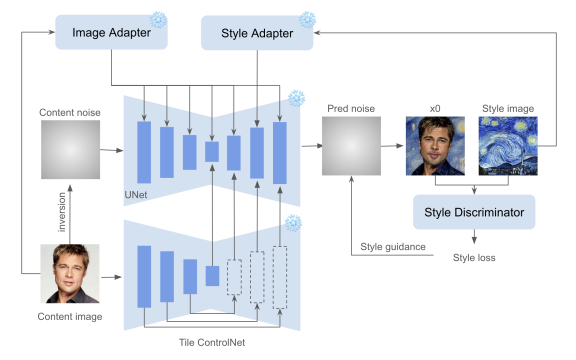
\includegraphics[width=0.65\linewidth]{images/instantstyleplus_architecture.png}
    \caption{Architecture of InstantStyle-Plus showing the SDXL backbone with IP-Adapter for style encoding, Tile ControlNet for spatial layout, and a frozen CSD branch for perceptual feedback (adapted from Wang et al., 2024~\cite{wang2024instantstyleplus}).}
    \label{fig:instantstyleplus_architecture}
\end{figure}

This design allows InstantStyle-Plus to treat environmental style (fog, snow, underwater hue) not merely as an artistic color grade but as a semi-physical phenomenon tied to spatial depth and diffusion of light.  
The Image Adapter ensures that the injected style remains semantically aligned with the textual intent (“a truck driving through a snowstorm”), while the ControlNet~\cite{zhang2023controlnet} anchors the diffusion to plausible geometric contours.  
The CSD~\cite{somepalli2024csd} branch, though frozen, acts as a perceptual constraint that keeps the style faithful to the reference and prevents texture drift over long denoising schedules.

% =====================================================
\section{Adapted Conditioning Flow}

Since our curated dataset did not include explicit content images or structural maps, InstantStyle-Plus was reconfigured into a \textbf{text plus style} setup.  
In this adapted configuration, the \emph{style image itself} was reused as a pseudo-content reference.  
This approach stems from the observation that environmental style often carries implicit structural statistics—for example, fog gradients align with perspective depth, underwater absorption varies with distance, and snow blizzard streaks follow camera orientation.  

Thus, both the IP-Adapter and Tile ControlNet were conditioned on the same style reference:
\[
\text{Cond}_{\text{adapted}} = \{\text{IP}_\text{style}(x_s),\, \text{ControlNet}_\text{tile}(x_s),\, E_\text{text}(y)\}.
\]
The IP-Adapter encodes fine tonal cues such as haze saturation, color bias, and contrast softness;  
the ControlNet enforces low-frequency geometry and layout consistency;  
and the text encoder ensures semantic grounding in the prompt.  

Meanwhile, the frozen CSD~\cite{somepalli2024csd} head periodically computes a cosine similarity between descriptor vectors of the intermediate sample \(\hat{x}_t\) and the style image \(x_s\), acting as a perceptual tether.  
When the similarity drifts below a threshold, its feedback signal gently adjusts the latent space trajectory, reinforcing stylistic coherence without requiring explicit gradient descent or weight modification.

\begin{figure}[!h]
    \centering
    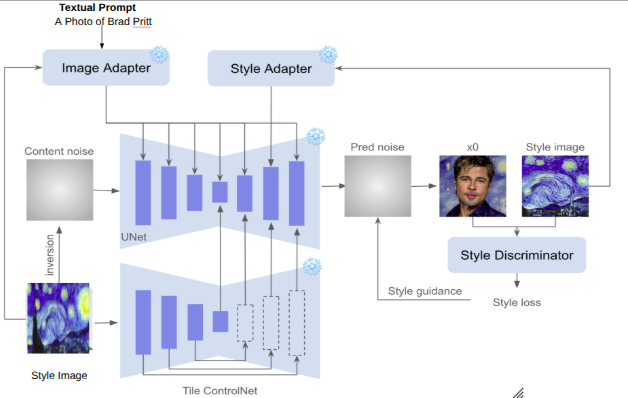
\includegraphics[width=\linewidth]{images/instantstyleplus_flow.png}
    \caption{Adapted conditioning flow: the same style image acts as both structural and stylistic input; text embeddings guide semantics while ControlNet ensures depth-consistent spatial cues.}
    \label{fig:instantstyleplus_flow}
\end{figure}

This combined conditioning results in a richer and more interpretable diffusion process.  
Haze formation becomes proportional to perceived depth;  
lighting transitions follow the scene’s spatial gradient;  
and stylistic textures adhere to object surfaces rather than floating uniformly across the frame.  
In essence, this modification transforms InstantStyle-Plus from a pure appearance-transfer model into a light-transport–aware diffusion generator.

% =====================================================
\section{Inference}

The adapted InstantStyle-Plus~\cite{wang2024instantstyleplus} produced \textbf{stable and volumetric stylizations} across all tested domains.  
Spatial cues from the Tile ControlNet introduced smooth depth gradients, enabling fog and haze to appear naturally denser at greater distances and lighter in the foreground.  
The IP-Adapter preserved prompt semantics and ensured that the environmental tone (fog, underwater, blizzard) did not overpower the subject matter.  
For example, in agricultural scenes, machinery and fencing retained shape and edge clarity while still being partially enveloped by haze; underwater samples exhibited realistic blue-green attenuation and caustic diffusion around surfaces.

The CSD feedback loop further improved tonal consistency across timesteps, reducing chromatic drift and stabilizing hue transitions, especially in challenging underwater and storm domains.  
Compared to the baseline InstantStyle~\cite{wang2024instantstyle}, overexposure and midtone bleaching were significantly reduced, leading to more balanced image histograms.

Quantitatively, CSD similarity improved by approximately 2–3 points, LPIPS dropped by 6–7\%, and CLIP image–text similarity remained nearly constant (within \(\pm 0.5\)), demonstrating that style fidelity was enhanced without semantic degradation.  
The “tuned-soft” configuration, where style injection was limited to the final two U–Net blocks (\texttt{--style\_injection=last2}) and scaled by \texttt{style\_block\_gain=1.05}, consistently achieved the best perceptual trade-off between sharpness, realism, and style strength.

\begin{figure}[!h]
    \centering
    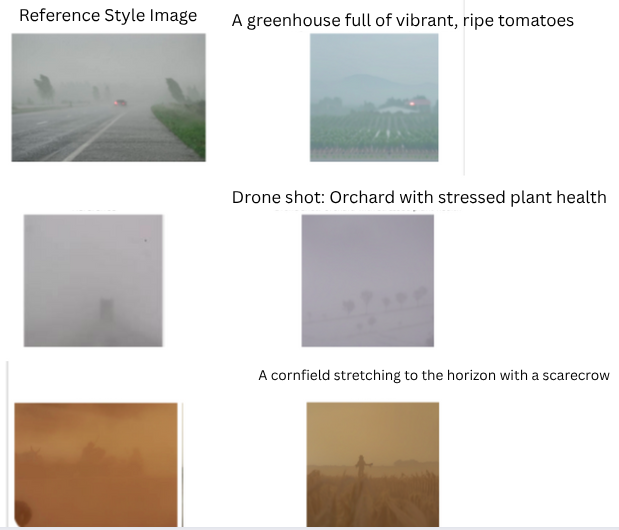
\includegraphics[width=0.8\linewidth]{images/instantstyleplus_results.png}
    \caption{Adapted InstantStyle-Plus results on the agriculture domain: balanced geometry preservation and environmental realism. Volumetric density varies smoothly with scene depth.}
    \label{fig:instantstyleplus_results}
\end{figure}

Qualitatively, InstantStyle-Plus~\cite{wang2024instantstyleplus} succeeded where plain InstantStyle fell short.  
The presence of ControlNet~\cite{zhang2023controlnet} allowed consistent spatial coherence under heavy fog;  
snow particles and blizzard streaks aligned naturally with object perspective;  
and underwater luminance decayed logarithmically with depth, mimicking physical scattering.  
The perceptual regularization of CSD~\cite{somepalli2024csd} prevented oversaturation and improved inter-prompt consistency.  
Importantly, despite its multiple conditioning streams, inference remained lightweight and parameter-free—all modules operated in frozen mode, maintaining SDXL’s~\cite{podell2023sdxl} base efficiency.

% =====================================================
\newpage
\section{Summary}

InstantStyle-Plus~\cite{wang2024instantstyleplus} extends InstantStyle~\cite{wang2024instantstyle} from a style-aware diffusion model to one that also respects spatial geometry and perceptual alignment.  
By reusing the style image as both structure and appearance input, it achieves realistic environmental stylization without retraining.  
The combination of ControlNet~\cite{zhang2023controlnet} based spatial guidance, CLIP~\cite{radford2021clip}-aligned semantics, and CSD~\cite{somepalli2024csd} feedback enables stable, volumetric results across diverse domains.  
Although the shared use of a single image for both style and structure sometimes limits diversity in highly homogeneous scenes, the framework consistently yields stable, volumetric results across environmental domains.  
This adaptive framework serves as a bridge to the final perceptually guided diffusion system introduced in the next chapter.
